\begin{wrapfigure}{l}{0pt}
  \centering
  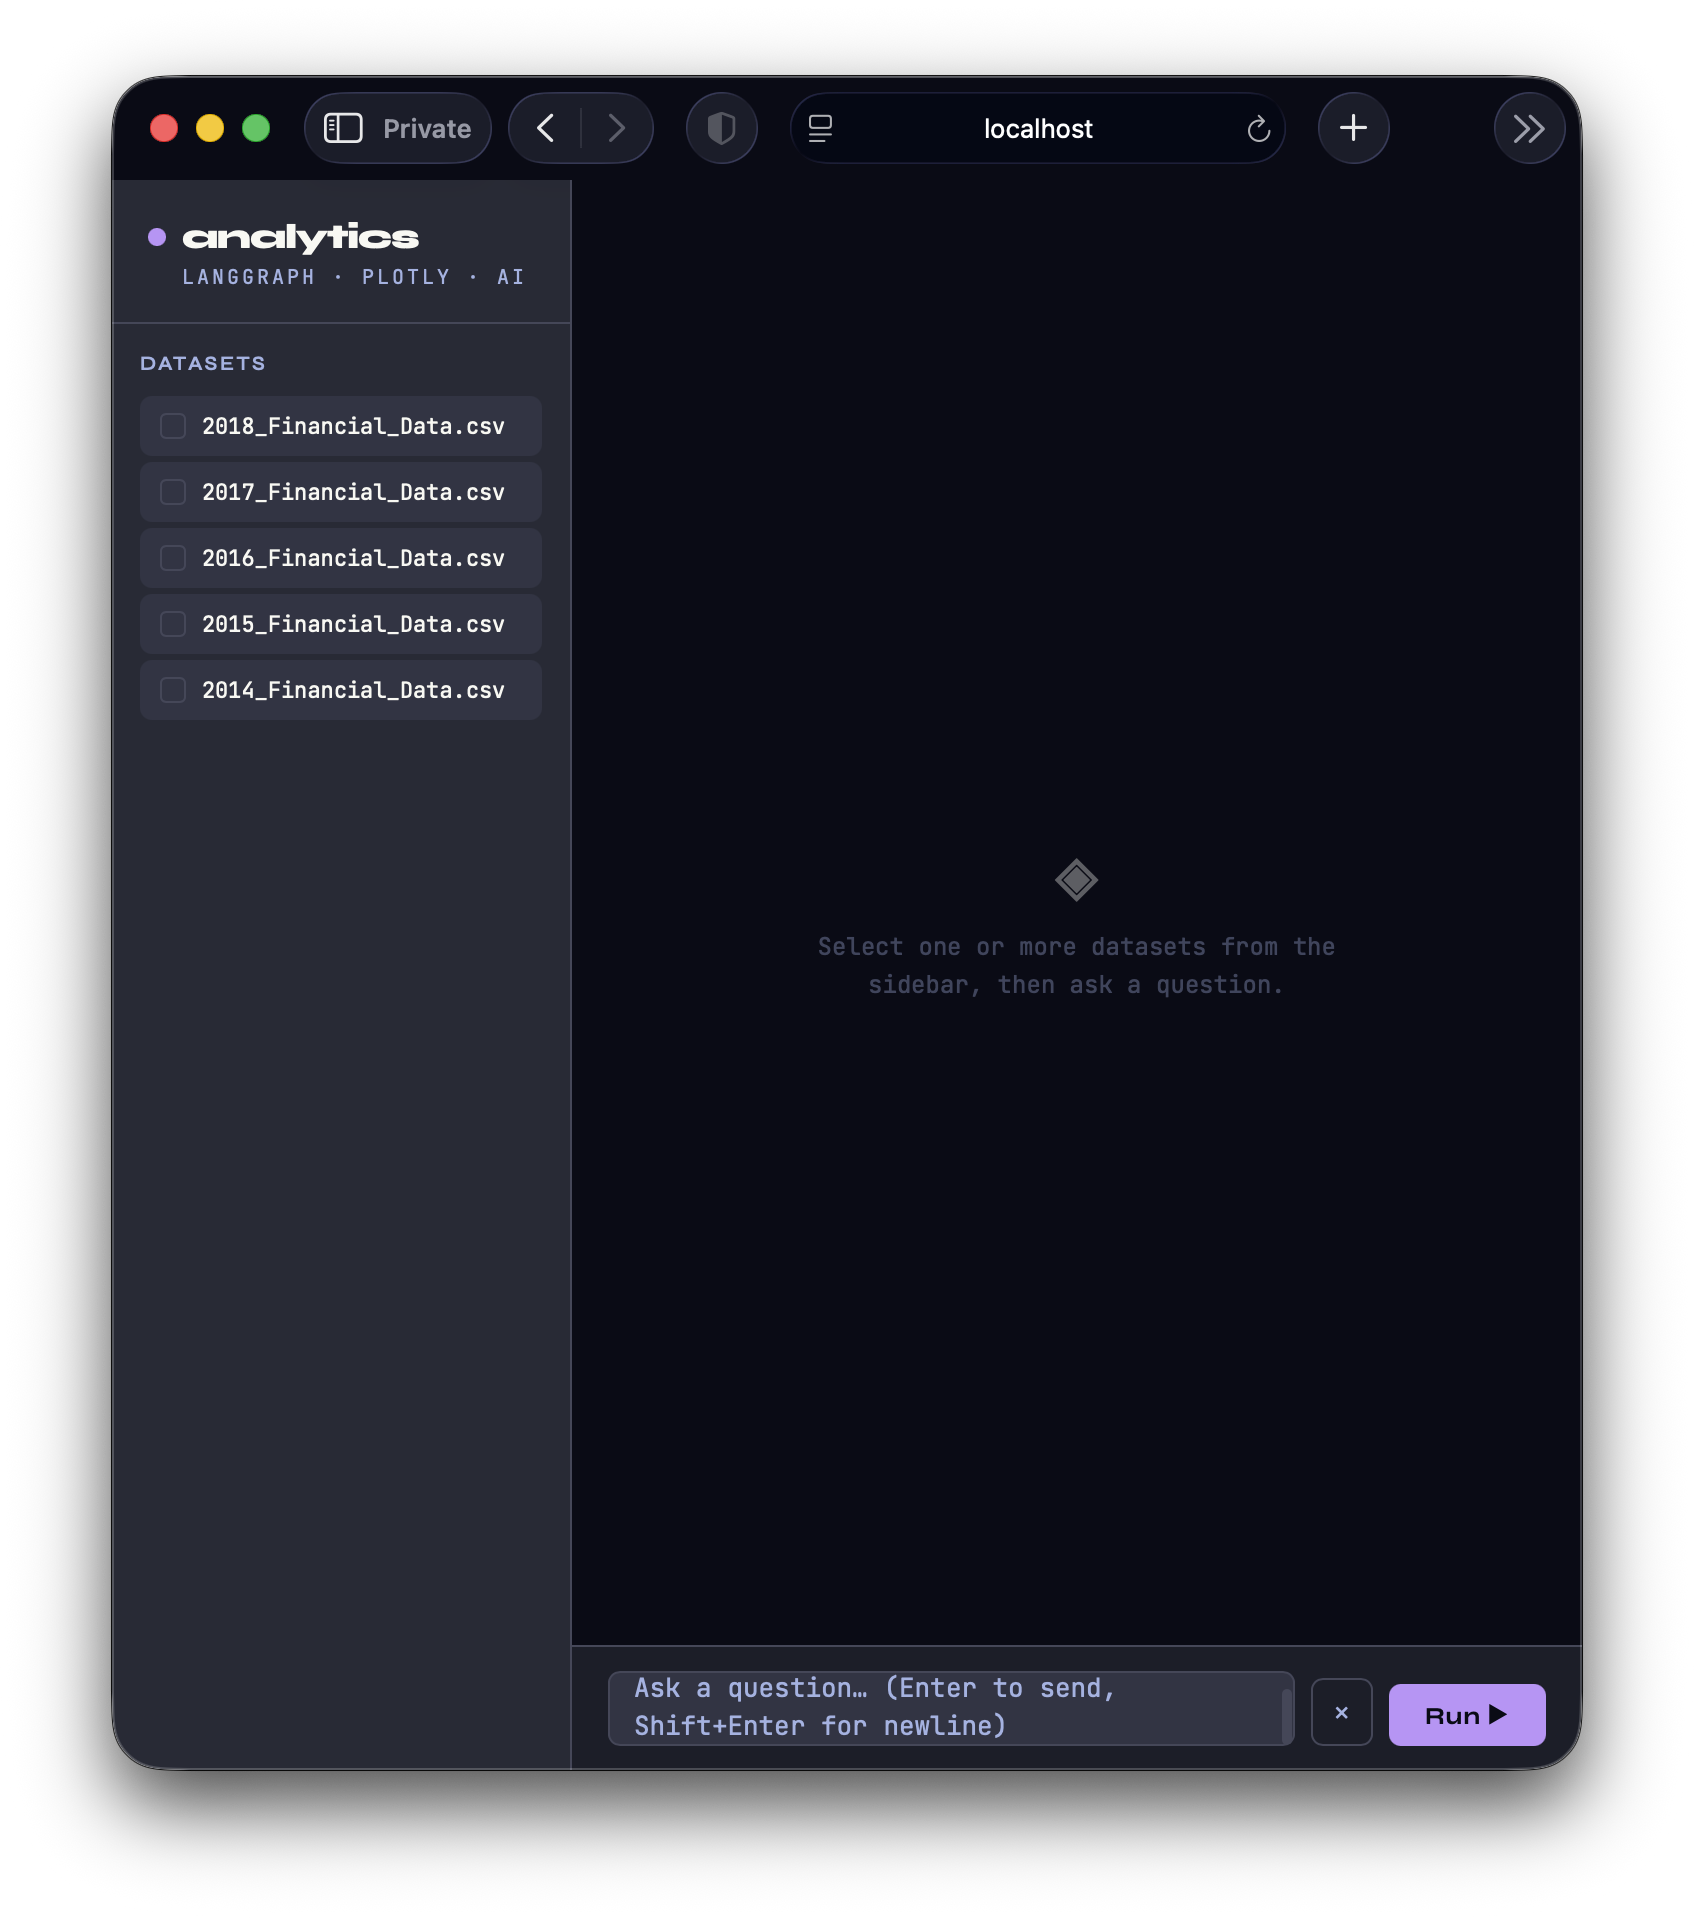
\includegraphics[width=0.4\textwidth]{graphics/ui-blank.png}
\end{wrapfigure}

The frontend is a single-page chat application served as a static HTML file by the FastAPI backend. The layout divides into two panels: a narrow left sidebar listing the available CSV datasets and a main conversation area. The user selects one or more datasets from the sidebar, types a question into the textarea at the bottom, and submits via the Run button or the Enter key.

All communication between the frontend and the backend uses Server-Sent Events (SSE). As the agent graph executes, the backend emits a stream of typed events — one per reasoning step, code block, plot, or final answer — and the frontend renders each incrementally as it arrives. This design means the user observes the agent's reasoning live rather than waiting for a completed response, which is particularly valuable for multi-step analytics queries that may take 15-30 seconds, or even minutes, end-to-end.

Each analytics step is rendered as a collapsible card labeled by step index. If the step involved Python execution, the card displays the generated code alongside its stdout output. Plots captured in the Plotly namespace are embedded as interactive figures using the Plotly JavaScript library. The validator verdict is rendered as a distinct badge — green for approved, amber for retry — before the final answer card is shown. Responses are rendered with Markdown support via \texttt{marked.js}, preserving headers, bullet points, and inline code from the model's output.
